
\documentclass[../main.tex]{subfiles}
\graphicspath{{\subfix{../images/}}}

\begin{document}
\section{Sampling and Descriptive Statistics}
\subsection{Sampling Methods, emphasis on Simple Random Sample}

\textbf{Definition:}\\
A \textbf{population} is the entire collection of objects or outcomes about which information is sought.
\\\\
A \textbf{sample} is a subset of a population, containing the objects or outcomes that are actually observed.
\\
Statistical methods are based on the idea of analyzing a sample drawn from a population. The sample must be drawn appropriately. The best sampling methods involve random sampling. 
\\\\
A \textbf{simple random sample (SRS}) of size n is a random sample of size n drawn from the population.
\\
SRS does not guaranteed to reflect the population perfectly. Two different samples from the same population will vary from each other as well, known as \textbf{sampling variation}.
\\\\
A \textbf{tangible population} consists of actual physical objects, it is always finite.
\\\\
A \textbf{sample of convenience} is a sample that is obtained in some convenient way, not well random.
\\\\
A\textbf{conceptual population} consists all values that might possibly have been observed from a population.
\\\\
The items in a sample are said to be \textbf{independent} if knowing the value of some items does not help to predict the value of others.\\
SRS are treated as independent in most cases. Except when population is finite and the sample comprises a substantial fraction($>5$\%) of the population.
\\\\
A \textbf{controlled experiment} is which the experimenter controls the values of the factors
\\\\
An \textbf{observational study} is where the experimenter simply observes the factors as they are, without having any control over them.
\\\\
The \textbf{sample mean} gives an indication of the center of the data.
\begin{equation*}
    \bar{X} = \frac{1}{n}\sum_{i=1}^{n}X_i
\end{equation*}
The \textbf{sample standard deviation} gives how variable the data are.
\begin{equation*}
    s^2 = \frac{1}{n-1}\sum_{i=1}^{n}{(X_i-\bar{X})^2}=\frac{1}{n-1}{\sum_{i=1}^{n}{{X_i}^2-n\bar{X}^2}}
\end{equation*}
\textbf{Resistant} is a statistic whose value does not change much when an outlier is added to or removed.
\\
Numerical summaries of a population are called \textbf{parameters}.
\\
Numerical summaries of a sample are called \textbf{statistics}
\\\\
\textbf{Other Sampling methods}:\\
- Weighted sampling\\
- Stratified random sampling\\
- Cluster sampling
\\\\
\textbf{Types of Data}:\\
- numerical or quantitative\\
- categorical or qualitative
\subsection{Histogram}
One peak: Unimodal\\
Two peaks: Bimodal\\
More than one peaks: multi-modal
\subsection{Box plot}
\begin{figure}[bh]
\centering
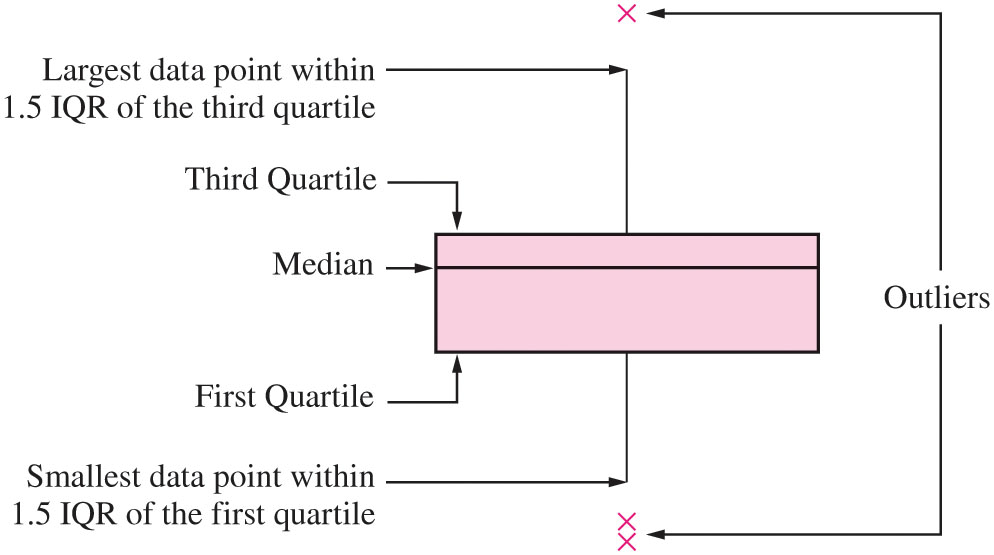
\includegraphics[width=10cm]{Sections/Image/BoxPlot.png}

\caption{Box Plot}
\end{figure}


\end{document}
